\documentclass[11pt]{article}
%Gummi|061|=)
\usepackage{hyperref}
\usepackage[spanish]{babel}
\usepackage[utf8]{inputenc}
\usepackage{pdfpages}
\title{\textbf{Diseño de Software: Klondike}}
\author{Sergio Arroutbi Braojos}
\selectlanguage{spanish}
\date{\today}
%\addtolength{\topmargin}{-0.5in}
\usepackage[bottom=14em]{geometry}
\usepackage{amsmath}
\usepackage{mathtools}
\usepackage{pdflscape}

\begin{document}

\hypersetup
{   
pdfborder={0 0 0}
}
   
\maketitle

\pagebreak

\tableofcontents

\pagebreak

\section{Introducción}
En este ejercicio se ha realizado el análisis, diseño y posterior implementación del juego del klondike. Este juego de cartas, también conocido como ``solitario'', es un juego en el que un único jugador interviene en el reparto y operación de las cartas. El tablero de cartas está formado por la baraja inicial, conocida como ``Deck'', el ``Waste'', donde se levantan las cartas de la baraja, una serie de ``Tableaus'', que permiten sacar de forma provisional las cartas del ``Waste'' ordenándolas por número descendente y alternando los colores de las cartas, y finalmente las ``Foundations'', que son cada uno de los palos del ``Deck'' en orden ascendente.

En cada turno, el jugador puede sacar cartas del ``Deck'' al ``Waste'', colocar cartas del ``Waste'' a los ``Tableaus'' o a las ``Foundations'' y sacar igualmente carta de las ``Foundations'' para seguir combinando cartas en los ``Tableaus''.
El motivo de este documento no es describir de forma muy detallada el juego, que puede consultarse en el siguiente enlace: \url{https://en.wikipedia.org/wiki/Klondike_(solitaire)}
Además, existen ciertas reglas que son configurables en el juego, como el número de cartas del ``Deck'' que se ocultan en cada ronda de la baraja al ``Waste'', el número de veces que el ``Waste'' se puede dar la vuelta hacia el ``Deck''.

Para realizar la implementación software de este juego de cartas se han realizado las diversas fases involucradas en el proceso de desarrollo unificado con diseño orientado a objetos. En este proceso se ha llevado a cabo la idea ``BDUF'' (Big Design Up Front), para el cual se han seguido las siguientes fases:

\begin{itemize}\itemsep0pt
\item{Captura de Requisitos}
\item{Análisis}
\item{Diseño}
\item{Implementación}
\item{Pruebas}
\end{itemize}

En los siguientes capítulos se describen cada una de las anteriores fases y la aproximación que se ha llevado a cabo con el objetivo de llegar a una implementación con un objetivo final: \textbf{Llegar a un software con un buen diseño orientado a objetos}, cuya mantenibilidad sea lo más sencilla posible, y caracterizado por las cuatro premisas que este tipo de diseño trata de alcanzar:

\begin{itemize}\itemsep0pt
\item{Abstracción}
\item{Encapsulación}
\item{Modularidad}
\item{Jerarquía}
\end{itemize}

Para ello, se ha procurado implentar una jerarquía de clases de la mayor calidad posible, caracterizadas por ser :
\begin{itemize}\itemsep0pt
\item{de Bajo Acoplamiento}. Es decir, tener poca relación de fuerza entre unas claes y otras.
\item{Cohesivas}. Por cohesión, nos referimos a la fuerza de ligadura entre los miembros de una clase.
\item{Suficientes}. Por suficiencia se entiende que la clase proporciona suficientes características para proporcionar lo que la abstracción supone cuando interactúe con ellas.
\item{Completas}. Las clases deben ser completas, de forma que capture todas las características que la abstracción supone de ellas.
\item{Primitivas}. De forma que las clases pueden ser implementadas de forma efectiva simplemente proporcionando acceso a las capas inferiores.
\end{itemize}

Con las anteriores características en mente se describe cada una de las distintas fases desarrolladas hasta la implementación final.

\pagebreak

\section{Captura de Requisitos}

Para la captura de requisitos no se ha seguido ninguna metodología especial. El hecho de que el juego Klondike esté ya documentado e implementado permite dar una idea del funcionamiento del mismo.

Por esto, la principal fuente de requisitos para el desarrollo del juego han sido, en este caso, la documentación existente:
Por otro lado, a modo de ``Hands-On'', se ha utilizado el juego ``aisleriot'', implementación del klondike en la distribución Ubuntu de Linux.
A parte de lo descrito anteriormente, se han presentado ciertas características adicionales que pueden suponer ``motivos de cambio'' a considerar en el diseño de la aplicación, como son:

\begin{enumerate}\itemsep0pt
\item{El juego debería estar basado en opciones de menú a través de texto}. Sin embargo, no debería resultar muy difícil el portado del juego para que tuviera interfaz gráfico.
\item{Se podrá cambiar de tipo de baraja (baraja de póquer/baraja española)}. En el caso en el que se utilice la baraja española, la aceptación de cartas en los ``Tableaus'' será por ``palo distinto'', en lugar de ``color distinto'', como ocurre con la baraja francesa.
\item{El diseño debería facilitar el poder cambiar el tipo de reparto de cartas en el Deal de forma sencilla}.
\item{El diseño debería facilitar que el número de Tableaus se pudiera modificar de forma sencilla}.
\end{enumerate}

\pagebreak

\section{Fase de Análisis}
La fase de análisis es, simplemente, un \textbf{``diseño preliminar''}. Se considera que esta fase de análisis se debe de llevar a cabo en una quinta parte del tiempo total respecto a la fase de diseño.

En esta fase de análisis, en el cual la solución al proceso de desarrollo empieza a tomar forma, se debe dar una primera visión interna del sistema, de forma que empiezan a aflorar los primeros diagramas estructurados por clases estereotipadas, y suele recoger aquellos detalles del dominio propios de los objetos tangibles del desarrollo en cuestión.

En esta fase se debe empezar a documentar en qué partes se va a descomponer el sistema de forma que se desarrolle una división del problema planteado en diversas clases que tendrán distintas responsabilidades e interactuarán entre sí para llegar a la solución final. En el caso del klondike, el análisis del sistema ha dado lugar a un diagrama estructurado como el que sigue: 

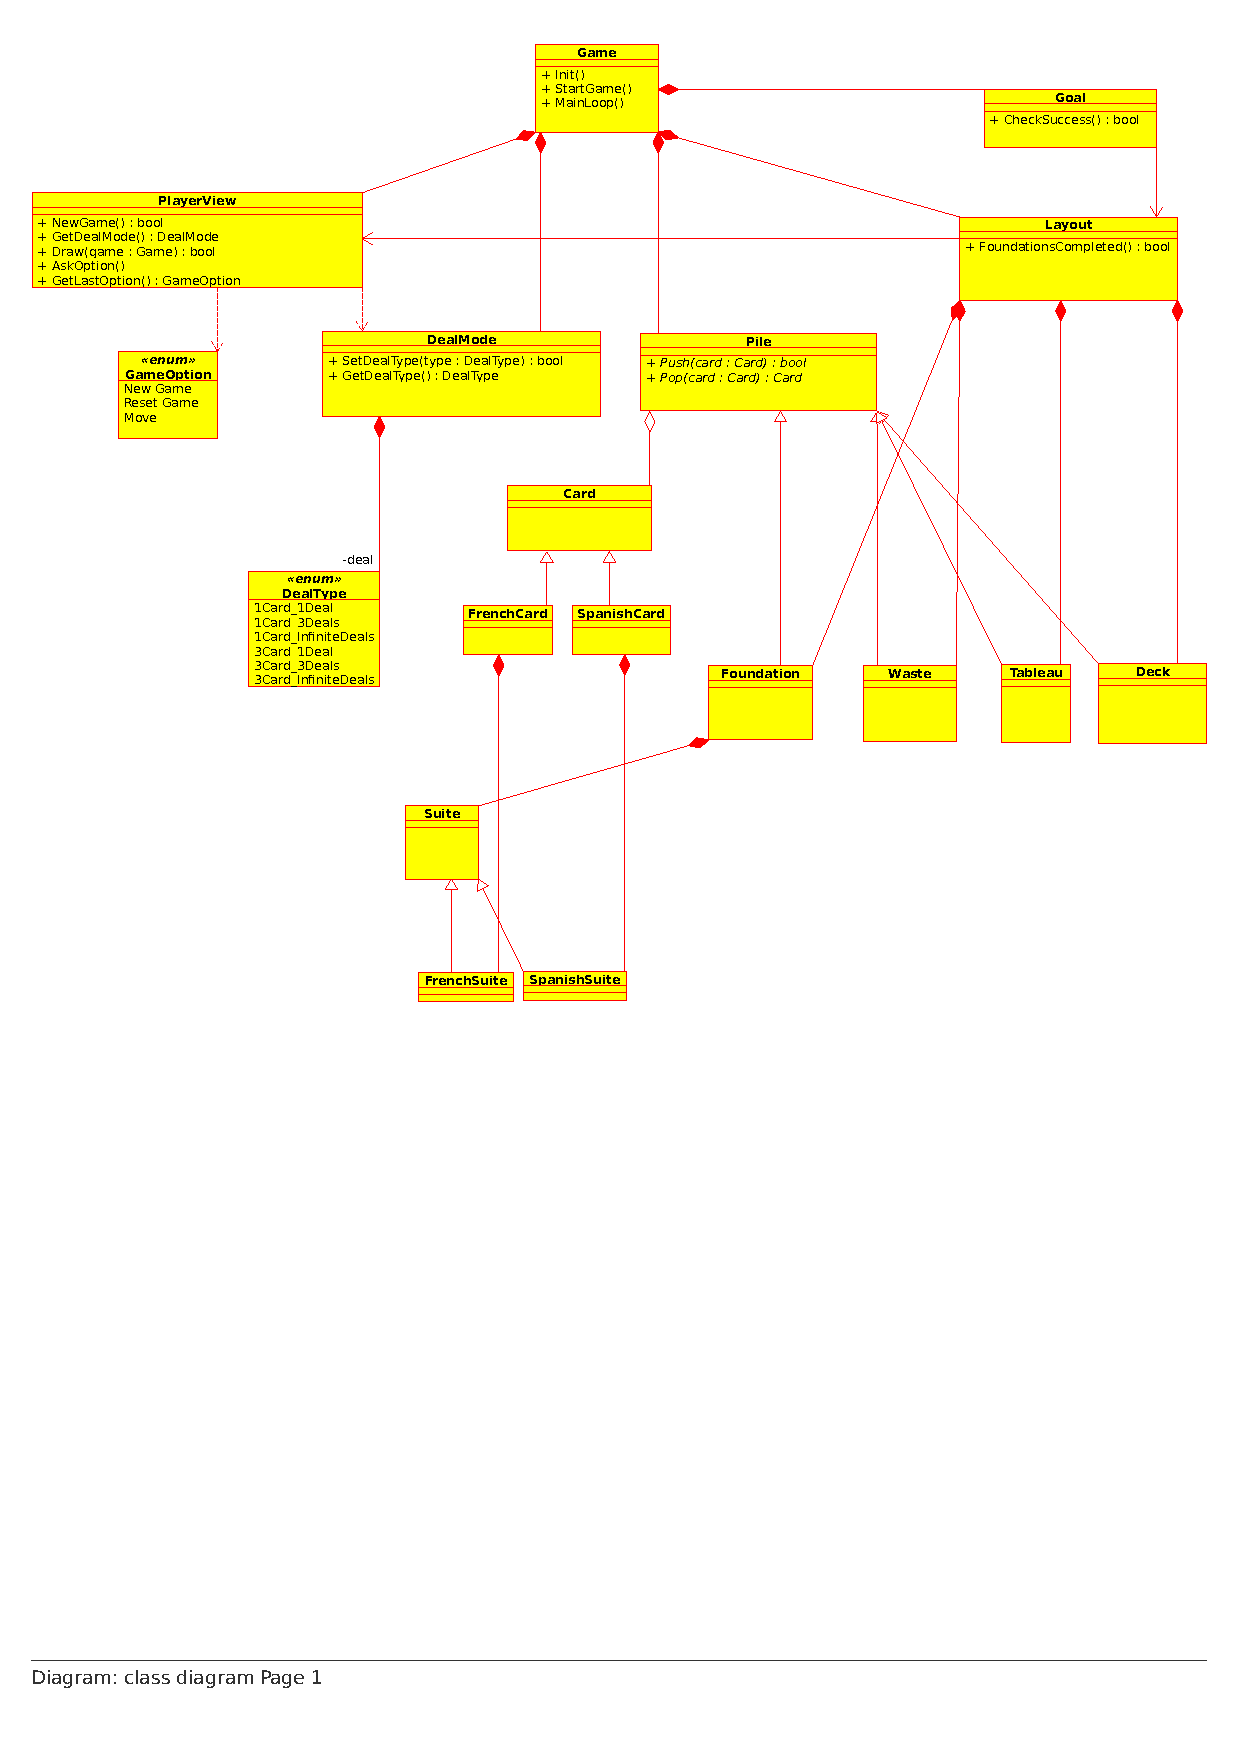
\includepdf[pages=-]{analysis00.pdf}

En este análisis preliminar se muestra un primer boceto de la jerarquía de clases. Normalmente, en esta fase de análisis, el diagrama de clases se centra en aquéllas que pertenecen al dominio del sistema. De esta forma, aparecen clases como "Deck", "Pile", "BoardLayout", "Game", etc. De esta forma, se han identificado en la fase de análisis los distintos tipos de clases que formarán la jerarquía que permitan implementar el juego.

A continuación se describe de forma resumida cada una de ellas:

\begin{itemize}
\item{\textbf{Game}}. Clase que contendrá el flujo principal de programa.
\item{\textbf{Goal}}. Clase encargada de chequear si ha terminado la partida.
\item{\textbf{PlayerView}}. Clase que se encargará de proporcionar al jugador la vista del juego.
\item{\textbf{DealMode}}. Clase encargada de mostrar los distintos tipos de reparto de cartas posibles.
\item{\textbf{Layout}}. Clase que contiene las estructuras de datos permtenecientes al tablero de juego, y, en concreto, a los distintos mazos de cartas que conforman el juego.
\item{\textbf{Pile}}. Clase padre de cada uno de los mazos específicos del juego. Recogerá las propiedades y métodos comunes de un mazo de carga.
\item{\textbf{Foundation}}. Clase que aglutina las propiedades y los métodos típicos de los mazos agrupados por colores que deben rellenarse por completo para ganar el juego.
\item{\textbf{Waste}}. Clase que modela el mazo en el que se sacan las cartas que provienen de la baraja.
\item{\textbf{Tableau}}. Clase para modelar cada uno de los mazos que se sitúan en la parte inferior del juego. Normalmente existen siete mazos de este tipo.
\item{\textbf{Deck}}. Clase que modela la baraja, situada en la parte superior derecha
\item{\textbf{Suite}}. Clase padre para modelar los palos de la baraja.
\item{\textbf{FrenchSuite}}. Clase para modelar los palos de la baraja francesa.
\item{\textbf{SpanishSuite}}. Clase para modelar los palos de la baraja española.
\item{\textbf{Card}}. Clase que modela una carta de la baraja. Típicamente tendrá un palo y un número.
\item{\textbf{FrenchCard}}. Clase que modela una carta de la baraja francesa.
\item{\textbf{SpanishCard}}. Clase que modela una carta de la baraja española.

Como puede observarse, en esta fase de análisis se pretende ir modelando la solución final, mediante una representación de aquellas clases del entorno del dominio en el que se sitúa el software a desarrollar.

En la fase de diseño, se acometerá el modelado completo de aquellas clases que se van a implementar, tanto aquellas que resultan del análisis del dominio como las que son resultado de la naturaleza intrínseca del software para acometer la resolución del problema final, en este caso, el desarrollo del juego del Klondike, también conocido como Solitario.
\end{itemize}

\pagebreak

\section{Fase de Diseño}

Como ya se comentó anteriormente, en la fase de diseño de software orientado se suele dedicar cinco veces el tiempo que se dedica en la fase de análisis. El objetivo final es realizar un diseño de clases que permita llegar a una arquitectura robusta. Para ello, el sistema debe cumplir una serie de características:

\begin{itemize}
\item{Flexibilidad}. El software del sistema debe ser sencillo de actualizar para incorporar nuevas funcionalidades.
\item{Robustez}. El software que compone el software debe ser robusto en cuanto a que no debe romperse por múltiples sitios cuando se realizan actualizaciones del mismo.
\item{Movilidad}. El software debe estar diseñado de forma que sea posible llevar partes del mismo (componentes) a otros sistemas, o bien para traer partes de otros sistemas a éste.
\item{Fluidez}. El software no debe ser viscoso, entendiendo como viscosidad aquella característica que hace que modficar una pequeña parte del software afecte a otras muchas partes.
\end{itemize}

Para cumplir con lo anterior, y llegar a una arquitectura sólida basada en un diseño robusto, el software debe cumplir una serie de principios, conocidos como "SOLID".

\begin{itemize}
\item{SRP (Single ResPonsability)}. Cada una de las clases debe cumplir un único cometido y tener una única responsabilidad, conociendo como única responsabilidad un único motivo de cambio
\item{OCP (Open Closed)}. Cada una de las clases debe proporcionar un interfaz abierto en cuanto a su comportamiento, pero a su vez cerrado en cuanto al soporte de la información que permite proporcionar dicho interfaz.
\item{LSP (Liskov's Substitution)}. Principio que establece que las precondiciones en las clases hijas deben ser menos restrictivos que aquellas de la clase padre, y a su vez que las postcondiciones de las clases hijas deben ser más restrictivas que las de la clase padre.
\item{DIP (Dependency Inversion Principle)}. Este principio establece que los módulos de orden superior no deben depender de módulos de menor nivel, sino que se deben establecer interfaces abstractos intermedios.
\item{ISP (Interface Segregation Principle)}. Principio que establece que los módulos únicamente deben heredar de interfaces que vayan a utilizar, en lugar de un interfaz extenso con ciertas partes que no utilizan.
\end{itemize}

A parte de estos principios, hay dos características primordiales que debe cumplir el sistema:
\begin{itemize}
\item{DRY(Don't Repeat Yourself))}. Característica primordial del software que establece que el software debe reutilizarse, y nunca copiar software en distintos módulos o internamente en un módulo, para favorecer su mantenimiento y no tener que modificar en más de un sitio para modificar una funcionalidad o arreglar un problema.
\item{KISS(Keep it simple)}. Característica que establece que se implementen clase y métodos sencillos para favorecer la reusabilidad y el mantenimiento del software.
\end{itemize}

El diseño propuesto en una primera iteración de la implementación se propone a través del siguiente diagrama de clases:

\newgeometry{top=0cm,left=1cm,bottom=0.3cm}
\begin{landscape}
\begin{center}
 \begin{figure}[H]
 \begin{center}
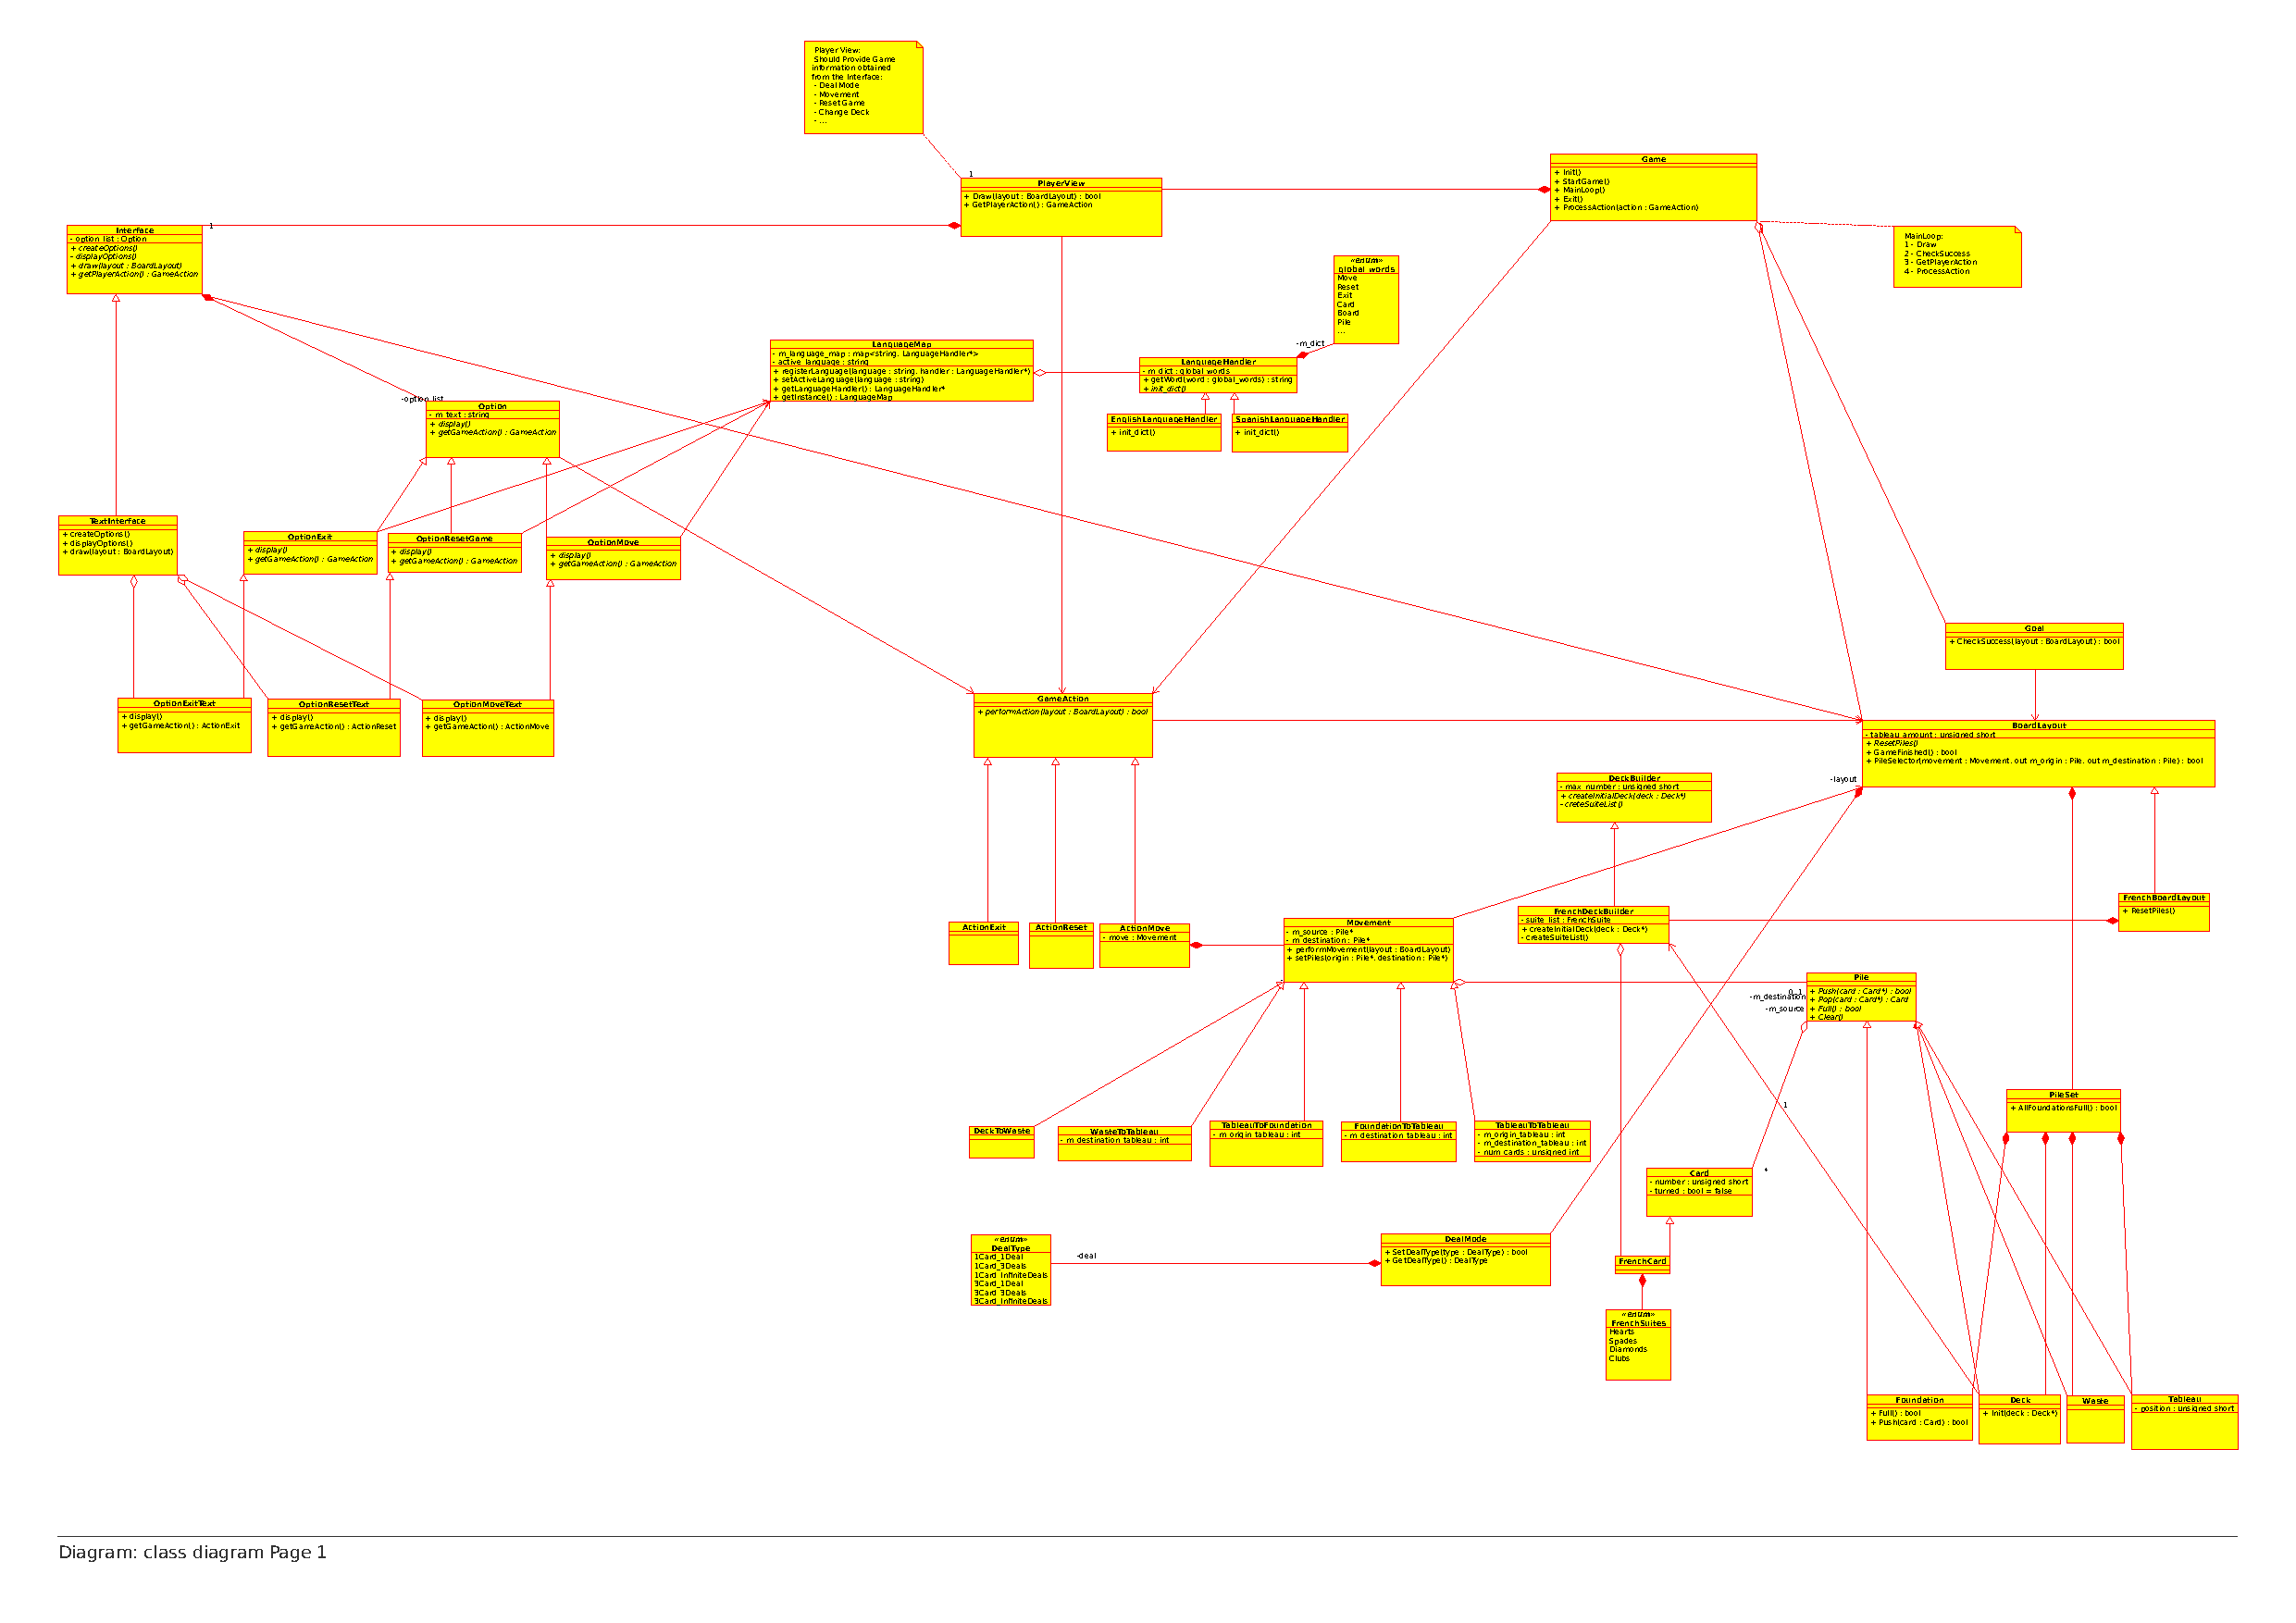
\includegraphics[scale=0.65]{design00.pdf}
   \label{fig:design}
 \end{center}
 \end{figure}
\end{center}
\end{landscape}
\restoregeometry

Como puede observarse, se trata de un diseño cuya máxima es mantener clases sencillas, principio KISS, que cumplan a su vez el principio SRP, en un diseño fuertemente jerárquico que permite el uso de las características de la orientación a objetos, como es el polimorfismo.

Mientras, el principio OCP está también presente en el diseño, de forma que las responsabilidades encapsulan el soporte de la información ocultando los objetos y/o atributos internos. Un ejemplo es la clase Movement, que permite encapsular los distintos movimienos posibles en el juego, ocultando el uso de las distintas pilas del tablero para acometer su responsabilidad.

Finalmente, y de forma principal, se ha evitado siempre tener que copiar y pegar código entre clases, ya que sus responsabilidades son muy distintas entre sí.

En esta primera iteración del diseño no se observan, sin embargo, otros principios, como pueda ser ISP. Además, este primer diseño, no recoge funcionalidad necesaria que no se contempló en un primer momento. 

Así, en una segunda iteración, el diseño final ha quedado como se muestra en el siguiente diagrama:

\newgeometry{top=0cm,left=2.5cm,bottom=0.3cm}
\begin{landscape}
\begin{center}
 \begin{figure}[H]
 \begin{center}
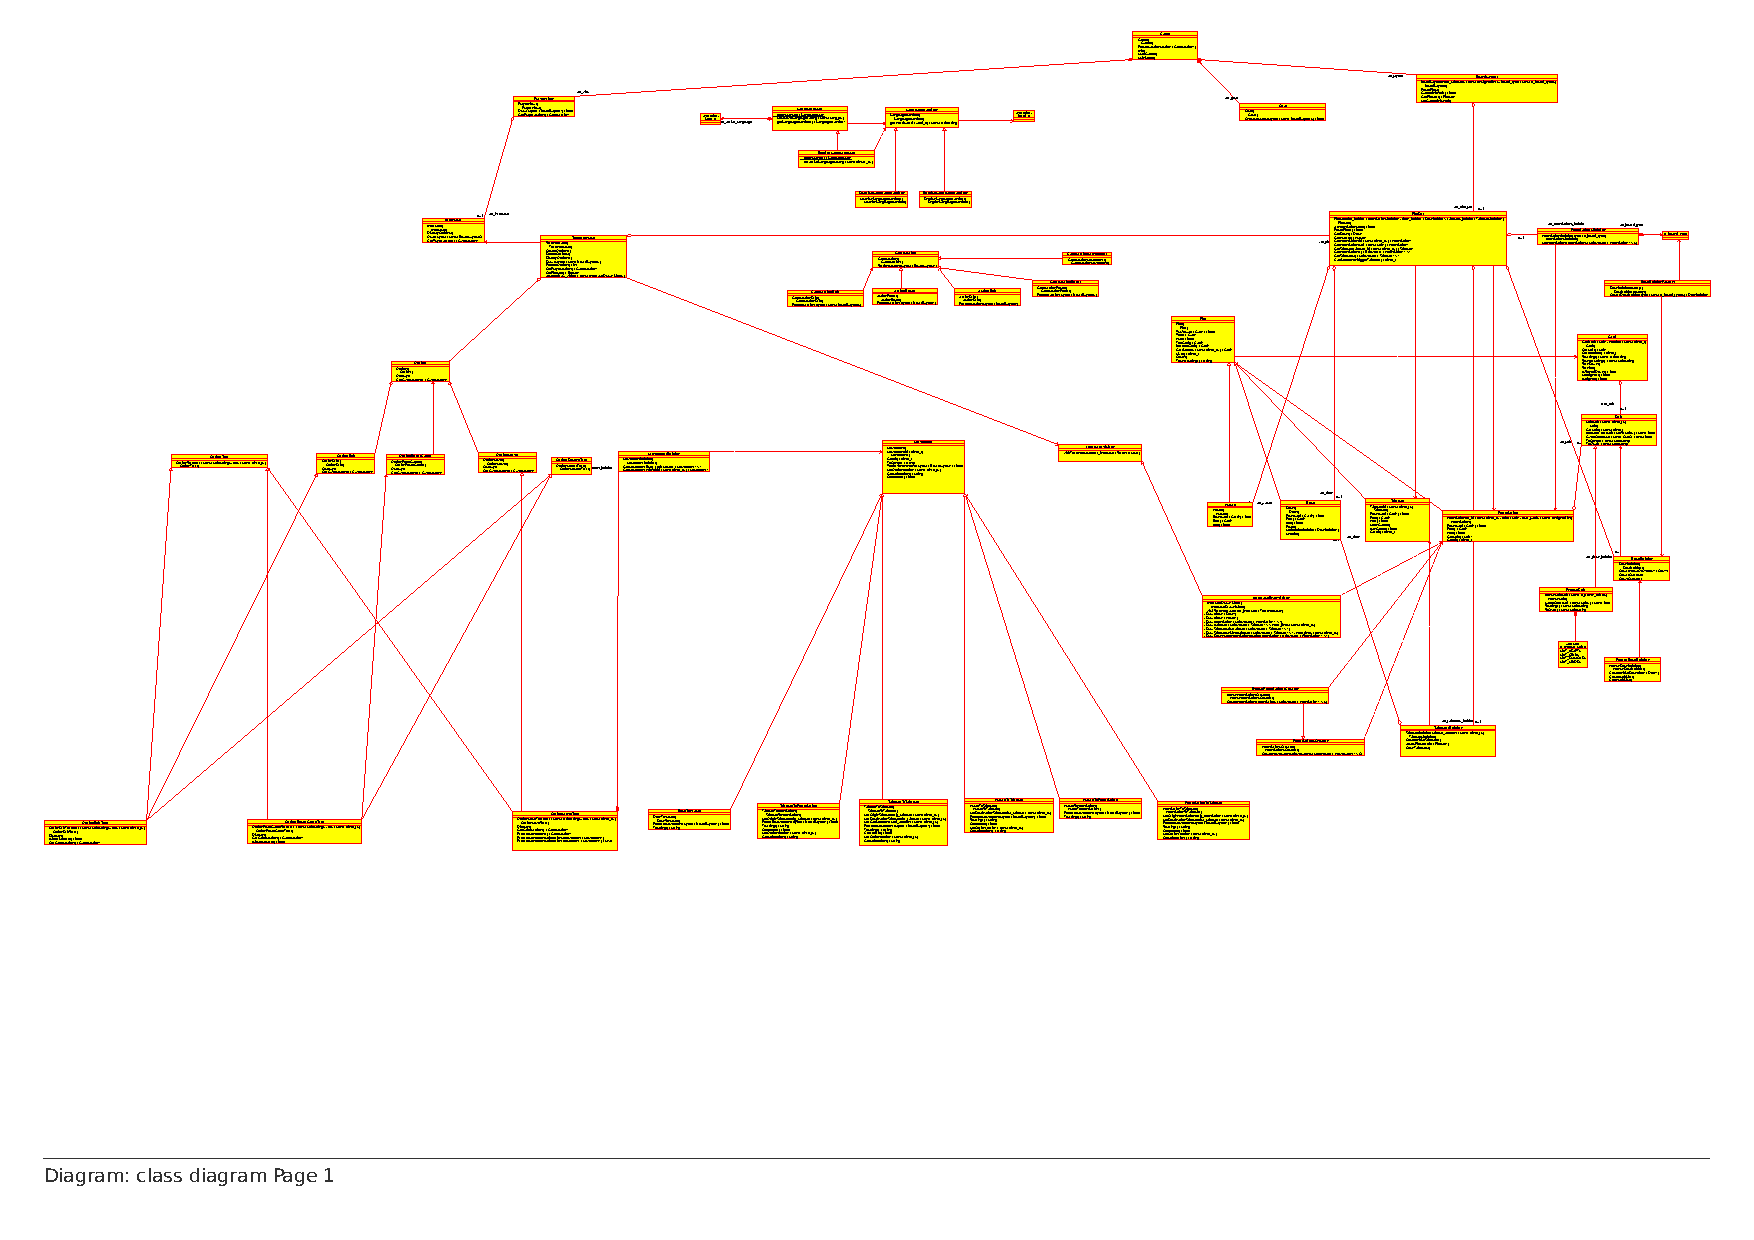
\includegraphics[scale=0.93]{final_design00.pdf}
   \label{fig:design}
 \end{center}
 \end{figure}
\end{center}
\end{landscape}
\restoregeometry

Este diseño mantiene las premisas de la primera iteración, pero incorpora básicamente:
\begin{itemize}
\item{Principio ISP}. Como puede observarse, por ejemplo, en las clases que heredan de la clase OptionSecureText, que son OptionExitText y OptionResetText, esto es, aquellas opciones que muestran texto por consola y que son las únicas que piden al usuario confirmación (Sí/No) debido a la importancia de las consecuencias de dichas opciones (salir del juego o bien reiniciarlo). Como puede observarse, las opciones que modelan los movimientos del tablero no necesitan confirmación del usuario, luego no heredan el interfaz OptionSecureText.
\item{Patrones de diseño}. En segundo lugar, este diseño final recoge una serie de patrones de diseño que se incorporan como soluciones recurrentes en el diseño ante problemas recurrentes que suelen aparecer en esta fase, como puedan ser la aparición de BLOBs (Big Large Objects), la necesidad de separar la creación de objetos de aquellos otros que los van a usar o a contener, o bien la necesidad de tener acceso global a objetos de multiplicidad única.
\end{itemize}

En el siguiente apartado se detallan los patrones de diseño utilizados y su justificación.

\subsection{Patrones de Diseño}

Los patrones de diseño describen soluciones estructuradas a problemas de diseño de software orientado a objetos que suelen ocurrir de forma recurrente. Normalmente, estas soluciones no se aplican de forma similar y suelen requerir modificaciones o combinaciones de patrones.

En el caso del desarrollo del sistema del juego del Klondike, se han introducido los siguientes patrones de diseño:

\begin{itemize}
\item{\textbf{Singleton}}. Para la gestión de órdenes que se emiten a través de pantalla, se ha decidido crear un LanguageMap que permita obtener una palabra o frase de forma transparente en función del idioma elegido. Este LanguageMap está compuesto por un mapa que debe inicializarse una única vez y, además, es un objeto que debe ser accedido desde varias partes del sistema. Luego la necesidad de tener un objeto de \textbf{referencia única y alcance global} hace que aplique este patrón.
\item{\textbf{Builder}}. El builder es un patrón creacional que permite separar la construcción de un objeto complejo de su representación. En la práctica del Klondike se han decidido crear distintos builders, para la baraja de cartas, DeckBuilder, para las fundaciones, FoundationBuilder, para los Tableaus, TableausBuilder y para los movimientos, MovementsBuilder. Este patrón se ha combinado con otro patrón creacional, la factoría de objetos, para crear según que Builders en función de parámetros como puedan ser, por ejemplo, el tipo de baraja utilizada.
\item{\textbf{Visitor}}. En un momento determinado del desarrollo se ha identificado una clase que estaba empezando a tener un número muy elevado de métodos. En concreto, en este desarrollo, ha ocurrido con la clase TextInterface, que permite mostrar por pantalla el juego a través de texto por la consola. Cuando esto ocurre, el patrón Visitor es útil para, a través de la técnica del doble despacho, eliminar atributos y/o métodos de la clase visitada y reducir su complejidad. En el caso del Klondike, se ha implementado un InterfaceDrawVisitor que permite pintar las pilas en pantalla visitando la clase TextInterface.
\end{itemize}

\pagebreak

\section{Fase de Implementación}

En cuanto a la implementación del código, se ha realizado en el lenguaje de programación C++. Si bien no se pretende en este documento entrar en demasiado nivel de detalle en cuanto a la implementación, cabe destacar que se ha procurado que el código cumpla una serie de premisas, sobre todo relacionadas con el principio KISS:
\begin{itemize}
\item{Clases sencillas}. Se ha procurado que las clases no sean demasiado grandes en cuanto a sus métodos y atributos. En el caso en el que se han identificado clases de este tipo, se han refactorizado partiendo en varias clases o aplicando patrones de diseño como el patrón Visitor.
\item{Métodos sencillos}. En cuanto a los métodos, se ha procurado que tanto su complejidad interna como su uso, entendiendo como tal el número de parámetros que contienen, sea el menor posible.
\end{itemize}

Por otro lado, se ha utilizado la herramienta "cccc", que permite obtener ciertas métricas que alertan sobre posibles riesgos existentes en el código, como puedan ser la complejidad ciclomática de los métodos, el acoplamiento entre objetos o el número de hijos que tiene una clase padre, entre otras. 

Se adjunta a la memoria el informe de esta herramienta en formato .html

\pagebreak

\section{Fase de Pruebas}

Si bien no era el objetivo de esta práctica, cabe destacar que, a parte de las pruebas manuales realizadas sobre el juego para depurar su funcionamiento, se han incluido pruebas unitarias. En este caso se ha utilizado la librería Google Test.

Se adjunta a la memoria la carpeta que contiene la definición de las pruebas unitarias.

\pagebreak

\section{Posibles Mejoras No Acometidas}

En cuanto a posibles mejoras que han quedado pendientes, se han identificado básicamente las siguientes:

\begin{enumerate}
\item{Patrones de Diseño}. Se ha identificado al menos un patrón de diseño adicional que se podría haber acometido. Se trata del patrón Composite, que hubiera permitido establecer, para un conjunto de cartas, un comportamiento similar a la hora de utilizarlas en comparación con una sola carta. Sería un patrón posible que se podría aplicar a la hora de mover cartas entre Tableaus, ya que puede moverse una única carta o bien un conjunto de más de una carta.
\item{Refactorización}. Si bien la herramienta utilizada para las métricas no identifica ninguna parte del código cuya complejidad sea muy elevada, sí que identifica dos partes que podrían ser refactorizadas:
\begin{itemize}
\item{Función PerformMovement, clase TableuToTableu}. Esta función posee un número de líneas de código y una complejidad ciclomática algo elevadas según la aplicación. Podría ser refactorizada.
\item{Clase BoardLayout}. Según la herramienta, existe un riesgo en el alto acoplamiento que tienen el resto de clases sobre ésta, ya que tiene muchas clases que dependen de ella (un total de 20). Estaría bien refactorizar el código para que, o bien se minimice el número de clases que la utilicen o bien se dote a la clase de una abstracción máxima para cumplir con las reglas de dependencia/abstracción entre clases.
\end{itemize}
\end{enumerate}
\pagebreak

\end{document}
